\documentclass[a4paper, 12pt]{report}
\usepackage{liner}

\title{\Huge the best way to count \\ \bigskip \Large soundtrack liner notes}

\author{Lucilla}
\date{}

\begin{document}

\vfill \maketitle \vfill \newpage

\newgeometry{left=4.25cm,right=4.25cm,top=5cm,bottom=5cm}

even though its primary purpose is to present arguments that there exists a base even better than base six, {\it the best way to count} is by no means meant to be any less nurtured in its musical aspect than its artistic project siblings that precede or follow it.

two central ideas guided the shape and style of the soundtrack as a whole. one was to have most of the songs in some way generated by a mathematical phenomenon, a concept only natural in a video essay about mathematics. thus the contents of every track except for {\it divide and conquer} and {\it dance of the symbols} are in a rather straightforward way made from mathemusical elements.

another leading premise was to give the musical aspect of the video essay a higher level of cohesion, not unlike that of a film score. the structure of {\it the best way to count} somewhat resembles a narrative; chapters 0~and~1 serve to introduce the ``main character'' and give them some time to expose a few character traits; 2~and~3 develop their story and make us follow their accomplishments as they grow stronger; 4~and~5 represent a crisis and downfall in power, the turning point of the plot, but one from which the character emerges victorious in the end; 6~and~7 are the after-party, the celebration of their final victory, the happy ending of the story. and so, while each piece of music adds to the big picture with its unique face, there also are a few overarching elements of unity, and the sense of elements fitting like puzzle pieces to assemble a greater whole.

the soundtrack even has what could be considered a kind of leitmotif, in the form of the so-called ``seximal theme'': the melody of Misali's {\it seximal fractions}, generated by concatenating the base-6 expansions of the reciprocals of small positive integers. fragments of it are scattered all across the video essay, from the jingles at the beginning of each chapter (which also indicate the chapter number in binary with their beats), through the Mario-style jingles separating the subsections in chapter 3, all the way to the melancholic introduction to chapter 7.

harmonically, the tracks are generally rather simple; they all stick to a single key, without venturing outside of it at all. the range of keys themselves is also basic, drawing only from the pool of the familiar {\sc c},~{\sc g},~{\sc d},~and {\sc a}. each track is tuned either to 12edo or JI, with each tuning receiving an equal share -- though some of the 12edo tracks feature a bit of microtonal bending.

one more element to the soundtrack is the occasional numerological mysticism. even though mathematics and numerology are as separate from one another as astronomy is from astrology, the idea of injecting secret messages into numbers is too alluring to resist it in a video whose focus is numbers.

the ``protagonist'' and ``antagonist'' of {\it the best way to count} are base two and six, respectively; their sum, $2 + 6$, is an elegant round number of items to count, but coincidentally also a power of two itself, and thus appears rather prominently.

there are $2 + 6$ chapters, of which the first six are the actual ``plot'' and the last two are a victorious celebration of its resolution. $2 + 6$ tracks in the album, of which the first six alternate between having names starting with a {\sc b} for ``binary'' and a {\sc d} for ``decimal'', and the last two start with other letters. $2 + 6$ points in the cube depicted on the album cover, of which six are visible forming a hexagon, while the other two are only implicit through the other lines that give it the appearance of depth -- a cover which, at first glance, represents seximal, much like the thumbnail of Misali's {\it a better way to count} appears to advocate for dozenal.

\begin{figure}[H]
	\centering
	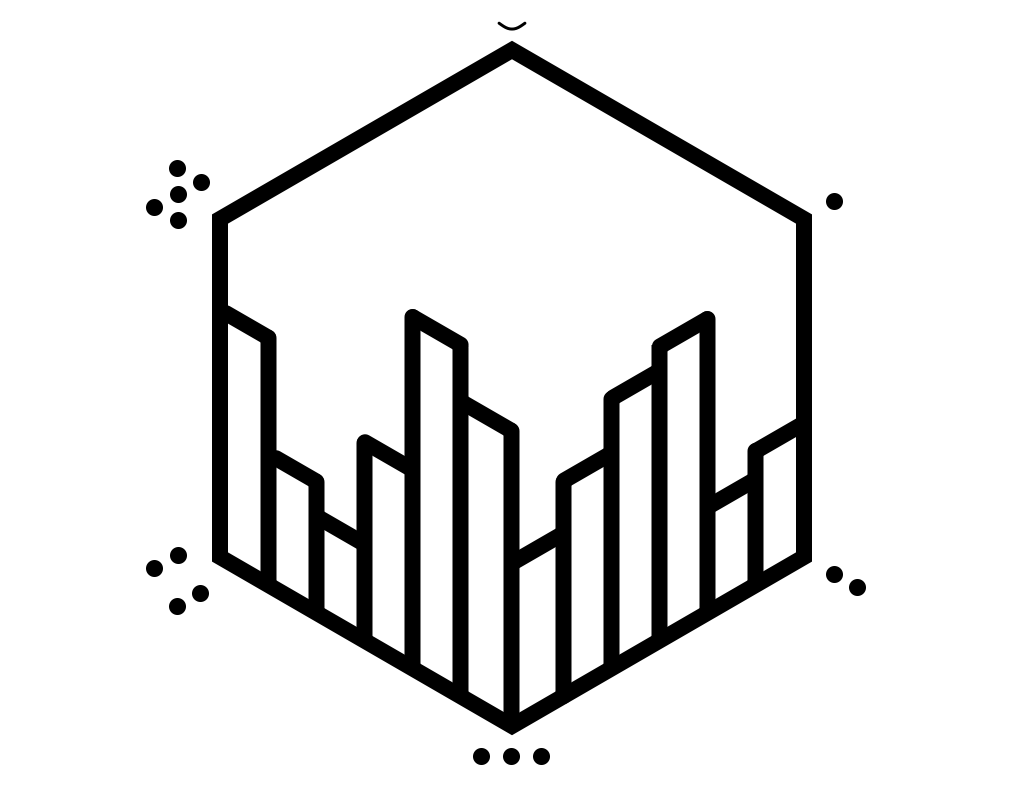
\includegraphics[scale=0.3]{cover.png}
\end{figure}

({\it ``binary'' would sound a lot prettier if it was instead named ``dyadic'' or ``dual'', but both of those would ruin the alternating alliteration.})

\restoregeometry

\newpage

\mysectionl{binary counter}{
	key: A -- tuning: JI -- plays in: chapter 2
}

a song that illustrates how binary counting is inherently musical to our ears. it begins as a mechanical implementation of a binary counter using sine waves, where the $n^{\text{th}}$ bit is a sine wave of frequency $n + 1$ times the fundamental ({\sc a$_2$}) -- which, when viewed in a visualizer that shows a spectrogram over time, will look like an actual binary counter. as it develops, it eventually turns into a full piece of music that counts all the way up to \io\jz\jo\jo\io\jo\jo\jo\io.

\mysectionr{decimal music}{
	key: G -- tuning: 12edo* -- plays in: chapter 3
}

Nystrom said introducing the decimal system into music would sound bad, and Lucilla took that personally: this song illustrates what music might sound like if rhythm was decimal. it counts from 0 to 1000 in ten verses, each of ten bars, each of ten notes, at 100 beats per minute. and it actually seems to have turned out pretty good, which ironically makes the point weaker, technically..?

at the very end, there's a {\sc g} major chord that fades into something strange. it's the nearest 10edo analogue of a {\sc g} major chord, the quantization of those notes to a system of \emph{ten} notes per octave instead of twelve, giving a glimpse of what it would be like if \emph{pitch} became decimalized too. (though remember that $n$-edo is really just powers of $2^{1/n}$, so it's really just binary all over again...)

\mysectionl{bach binary}{
	key: C -- tuning: 12edo* -- plays in: chapter 7
}

this track is a binary take on Bach's famous {\it Prelude in C Major}, BWV \jo\io\jz\jo\jz\iz\jo\jo\jo\iz. almost the entire prelude simply consists of chords, so it's possible to rearrange the notes so that every bar is a 4-bit binary counter. the number of bars that have this pattern happens to itself be a power of two ($2^5$), making the entire piece a 9-bit binary counter.

the melody in the first half of the piece comes from Charles Gounod's {\it Ave Maria}, while in the second half it just does its own thing. the ending is a reference to P.~D.~Q.~Bach's {\it Short-Tempered Clavier}, with some slightly pitch-bent blue notes.

\mysectionr{divide and conquer}{
	key: D -- tuning: JI -- plays in: chapters 4 \& 5
}

this short track, the only one in a minorish key, accompanies what at first glance appear to be the failures of binary. it's inspired by Arvo P\"art's {\it Fratres}, and is written using its characteristic ``tintinnabuli'' style over the gamelan-like pentatonic scale {\sc d}, {\sc e}, {\sc f}, {\sc a}, and {\sc b}-flat, where the middle voice only uses the notes of a minor triad: {\sc d}, {\sc f}, and {\sc a}.

in accordance with the track's role in the video essay, the animation accompanying it in the music video is a series of scrolling lengths of fractions in seximal and binary, marking the line in red whenever its length corresponds to a cyclic number. this is the argument that {\it seximal responses} presents to dispel binary -- and this is the argument we must deconstruct.

the name of this track is an elusive pun. ``divide and conquer'' is an idiom, but it also refers to what seximal allegedly does: it ``divides'', i.e. has more divisors, and therefore ``conquers'' binary.

\mysectionl{byteplex}{
	key: D -- tuning: JI -- plays in: chapter 1
}

alludes to Adam Neely's idea that ``polyrhythms are polypitch''. indeed, chords are just really fast polyrhythms, and here, every chord is also simultaneously its corresponding polyrhythm: each note's pitch frequency is also its rhythmic frequency, and in the animation, also the length of its corresponding line. the last measure features the raw polyrhythm corresponding to a major triad, $4:5:6$.

\mysectionr{dance of the symbols}{
	key: D -- tuning: 12edo -- plays in: chapter 6
}

a short neo-Romantic piano piece, in the style of a folk dance in triple meter. it accompanies the spoken names of binary numbers from 0 to $2^8$ as they scroll by, using to its advantage the coincidence that 4, a power of two, can be represented as the sum of powers of three, as $1 + 3$.

\mysectionl{magic sequences}{
	key: C -- tuning: JI -- plays in: introduction, chapters 4 \& 5
}

the ``title theme'' of this video essay, this is the response to Misali's {\it seximal fractions}: a track based on turning binary fractions from $1/2$ to $1/32$ into music. at first glance this might seem impossible, since unlike in seximal, binary fractions only have two possible digits, so there'd be no melodies. but you simply have to think outside the box a little and use the magic sequences \emph{themselves} as the basis instead. this actually ends up making it easier to convert the numbers into pitches: you don't need to pick any arbitrary scale, you just choose a fundamental frequency ({\sc c$_2$} in this case) and every number $n$ is simply represented by the note $n$ times that frequency. and it sounds good too, ...at least as long as it doesn't get too microtonal (though at that point, beyond 16, the melody gets some extra harmonization to make it more credible to the musically gullible).

but apart from that, this mapping has several benefits: \bigskip

\begin{itemize}
	\item using silence for 0 actually makes sense here, since a sound of frequency zero is silence -- unlike in {\it seximal fractions}, where it's an exception, and following the rule strictly would lead to 0 becoming the {\sc b} below middle {\sc c}: an off-by-one error.
	\item since the start and end points of a magic sequence's period are unambiguously determined by its entries (if it ends in a note that has already occurred before, then it loops at that note; if it ends with no duplicates, then all remaining entries are 0), repetition is optional and can be used freely for musical effect, as in the case of 11 and 13 -- unlike in {\it seximal fractions}, where an arbitrarily chosen number of repetitions is required to encode the message that the pattern repeats forever, possibly with ambiguity.
	\item binary magic sequences always start with powers of two, and contain many instances of doublings. but doubling a frequency means raising a note by an octave, so this is transparently audible in the music as sequences of rising octaves. due to octave equivalence, the magic sequences for $n$ and $2n$ sound almost exactly the same.
	\item the choices for the pitches are, in a way, more natural than pitches that come from an arbitrary scale that sounds good ``by design'', like the major scale. this alludes to how binary is more natural in a way than any other base, including those that work good ``by design'', like seximal.
\end{itemize}

\newpage

\mysectionr{sexim alive}{
	key: A -- tuning: 12edo -- plays in: credits, trailer
}

the final piece in the soundtrack, accompanying the home stretch after everything has been vanquished, is a setting of the theme from {\it seximal fractions} into a musical reprise that unfolds as the credits roll.

apart from here, the ``seximal theme'' -- consisting of the seximal expansions of small fractions -- appears throughout the video essay in small fragments, but only ever going up to $1/11$, and often only up to $1/5$. this song is the only place where they continue for much longer and venture into far further territory.

this song was changed as a nearly last-minute step in development. originally, it was a blend of the melody of {\it seximal fractions} with the structure and chords of the credits song from Portal, {\it Still Alive}: hence the song's name. more lively and cheerful, it would probably have crowned the ending of the video essay better than the more mysterious and contemplative new version -- alas, YouTube's automated copyright claim algorithm is aggressively merciless, and the song needed to be rewritten in the nick of time to remove the evil reference. the original can still be heard in the video essay's trailer, and is included on Bandcamp as a bonus track.

featured seximal fractions include: \bigskip

\begin{itemize}
	\item $1/2$ through $1/11$,
	\item $1/13$ through $1/17$,
	\item $1/19$,
	\item $1/25$,
	\item $1/29$,
	\item $1/36$,
	\item $13/22$,
	\item $79/132$,
	\item $4241/7776$,
	\item $157/288$.
\end{itemize}

\bigskip

figuring out where those fractions that aren't reciprocals of positive integers occur in the song is left as an exercise to the listener.

\newpage

\newgeometry{left=4.25cm,right=4.25cm,top=5cm,bottom=5cm}

\vspace*{\fill} \centering

{\bf the best way to count OST} \smallskip \\
\jo\jo\io\jo\jo\jo\iz\jz\jo\jo\iz---\,\jo\jo\io\jo\jo\jo\iz\jz\jo\jo\io \\
composed, mixed \& mastered by Lucilla \bigskip

attribution 4.0

\end{document}
